\section{Combinaison des deux modèles}
\subsection{Décomposition du problème}
\subsubsection{Pourquoi décomposer le problème en éléments simples}
Il s'agit à présent de partir du problème initial, de le découper en sous-éléments qu'on sait résoudre grâce aux méthodes présentées précédemment, puis de recombiner ces sous-éléments.\\
Partons du modèle de la grille, qui modélise le hangar (en figure \ref{fig:grille1}).\\
\begin{figure}[h]
	\centering
	\includesvg[height=5cm]{grille1}
	\caption{Modèle du hangar avec les points imposés de la trajectoire}
	\label{fig:grille1}
\end{figure}
\paragraph{Application directe de Dijkstra}Une approche naïve consisterait à appliquer directement l'algorithme de Dijkstra à toute la grille. Pour modéliser cette grille, il faut construire un graphe non orienté à arêtes valuées. Pour notre problème, chaque arête doit représenter un unique chemin, et sa valuation le temps parcouru.\\
Or 5 segments consécutivement alignés, ce n'est pas la même chose que 5 segments consécutivement perpendiculaires: le modèle mécanique nous dit qu'on va être obligé de ralentir avant de prendre chaque virage. Ces deux chemins auront donc une valuation différente. Ils seront donc représentés par deux arêtes différentes. Dans certains cas, il y a donc plus d'arêtes que de segments de couloir. On ne peut donc pas appliquer directement Dijkstra à la grille, ce n'est pas le graphe que l'on souhaite, il faut opérer une transformation, ou utiliser un algorithme plus adapté. C'est ce que nous verrons plus loin.\\
L'impossibilité d'appliquer directement Dijkstra peut être vue différemment. Ce qui nous intéresse, c'est de choisir le meilleur chemin passant par les différents points imposés.En supposant qu'il n'y ait pas de grille, on pourrait relier les points par des segments de droite, valués par leur longueur ou leur temps, et directement appliquer Dijkstra. Mais la grille impose un chemin le long de ses couloirs, donc on ne peut pas assimiler le graphe à l'ensemble des points imposés et les relier, puisque la ligne droite n'existe plus, et qu'il existe plusieurs moyens d'aller d'un point imposé à l'autre, et que certains sont meilleurs que d'autres. Si on voulait énumérer l'ensemble des chemins possibles, on obtiendrait un graphe avec beaucoup plus d'arêtes que de segments de couloir. Ce qui fait qu'on doit calculer un très grand nombre de valuations. Il est donc impossible d'appliquer directement Dijkstra à la grille.

\subsubsection{Algorithmes locaux}
Nous allons partir d'un algorithme naïf, qu'on va tenter d'améliorer. On va ensuite partir d'une heuristique, et montrer qu'elle est quasiment toujours optimale.
\paragraph{Par énumération naïve}Pour éviter une énumérations de tous les chemins préalable à leur valuation: on va faire cette énumération de façon plus locale, seulement là où on en a besoin. En effet, si on sait à l'avance qu'un segment de couloirs ne fera jamais partie d'un chemin optimal, il est inutile de calculer l'ensemble des chemins passant par ce segment. Une condition suffisante (mais pas nécessaire) permettant d'affirmer qu'un segment de couloir ne fera jamais partie d'un meilleur chemin entre deux points imposés, est de vérifier s'il appartient à la grille de taille minimum contenant les deux points imposés. Dans la figure \ref{fig:grille2} on montre un exemple de segment de couloir qui ne peut constituer un chemin optimal.\\
\begin{figure}[h]
	\centering
	\includesvg[height=4cm]{grille2}
	\caption{Le chemin rouge ne peut être un chemin optimal entre A et B, car il sort de la grille verte délimitée par A et B}
	\label{fig:grille2}
\end{figure}
Une fois qu'on a réduit l'étude des chemins possible à ceux de la sous-grille, il devient plus raisonnable d'énumérer tous les chemins. On a commencé à dessiner des chemins entre A et B en figure \ref{fig:grille3}.\\
\begin{figure}[h]
	\centering
	\includesvg[height=4cm]{grille3}
	\caption{On commence à énumérer les chemins dans la sous-grille délimitée par A et B}
	\label{fig:grille3}
\end{figure}

Pour encore améliorer ce traitement, on peut aussi enlever les arêtes qui ne vont pas jusqu'à B. On obtient alors un graphe non traitable par un Dijkstra, avec un algorithme mauvais, mais qui a été appliqué localement donc sur des données de taille raisonnable. On peut voir un exemple de résultat en figure \ref{fig:grille4}.\\
\begin{figure}
	\centering
	\includesvg[height=4cm]{grille4}
	\caption{On énumèré tous les chemins possibles; c'est un mauvais algorithme, mais il est appliqué sur de petites données.}
	\label{fig:grille4}
\end{figure}
\paragraph{Par minimisation des virages}
L'idée de la décomposition en sous-problèmes locaux est bonne, mais l'algorithme d'énumération utilisé dans chaque sous-problème local est très mauvais.\\
On peut le remplacer par un algorithme beaucoup plus puissant, mais pas forcément exact, en faisant une hypothèse: en supposant qu'une ligne droite est forcément plus rapide qu'un virage. Nous discuterons de la validité de cette hypothèse plus bas. En la supposant vraie, on n'a plus qu'à minimiser le nombre de virages, il suffit de construire la plus grande ligne droite, donc de parcourir la sous-grille par l'un de ses deux côtés (voir figure \ref{fig:grille5}). On a ainsi une heuristique très simple et très puissante permettant de calculer un bon chemin pour tout couple de points, qui est le meilleur chemin lorsque l'hypothèse est vraie.\\
\begin{figure}
	\centering
	\includesvg[height=6cm]{grille5}
	\caption{Entre deux points de la grille, il n'existe que deux chemins minimisant le nombre de virages.}
	\label{fig:grille5}
\end{figure}
L'hypothèse peut être formulée ainsi: pour tout couple de chemins de même longueur (en distance), le chemin le plus court (en temps) est celui qui a le moins de virages.\\
Cette hypothèse est bien suffisante à l'heuristique qu'on vient de présenter, puisque pour chaque couple de points imposés, tous les chemins de la sous-grille optimale reliant ces deux points sont de même longueur.\\
Mais est-elle toujours vraie?\\
Intuitivement, on pourrait penser que cela dépend de la largeur de la grille et du modèle mécanique. Si la grille est suffisamment fine (càd. la longueur d'un couloir est suffisamment petite), ou si le chariot est suffisamment agile dans un virage (càd. capable d'accélerer suffisamment dans un virage sans se renverser) alors on pourrait être dans un cas où la longueur de deux couloirs alignés n'est pas suffisante pour que le chariot accélère suffisament pour dépasser la vitesse qu'il aurait dans un virage. Dans ce cas, prendre plusieurs virages pourrait être plus efficace.\\
Mais nous allons montrer que ce modèle est faux, en prenant le cas extrême. Supposons que la vitesse en ligne droite est constante, et suffisamment basse pour que le chariot n'aie pas besoin de ralentir avant de prendre un virage. On peut voir un exemple en figure \ref{fig:grille6}.
\begin{figure}
	\centering
	{\small \includesvg[height=5cm]{grille6}}
	\caption{Le cas extrême: la vitesse en ligne droite est constante et ne nécessite pas de ralentissement avant le virage}.
	\label{fig:grille6}
\end{figure}
Alors dans ce cas, la seule différence entre deux chemins de la sous-grille est le nombre de virages. Or, les virages ont eux-même un coût en temps non-nul. Dans ce cas, la différence en temps entre deux chemins est proportionnelle à la différence en nombre de virages.\\
En pratique, il y a également une accélération sur une ligne droite qui permet d'aller encore plus vite; c'est illustré en figure \ref{fig:grille7}.
\begin{figure}
	\centering
	{\small	\includesvg[height=4cm]{grille7}}
	\caption{Un cas réaliste}
	\label{fig:grille7}
\end{figure}
Finalement, on peut donc utiliser cette heuristique dans tous les cas.
\subsection{Recombinaison des solutions locales et application du modèle mécanique}
On a donc montré que notre heuristique locale était valable quel que soit le modèle mécanique (à condition d'utiliser une grille). Quel que soit le couple de  points imposés, on peut donc déterminer un chemin optimal entre ces deux points. Il s'agit à présent de tracer tous les chemins localement optimaux, puis d'appliquer Dijkstra au graphe ainsi obtenu.\\
Le nombre d'arête est donc $\frac{n(n-1)}{2}$ où $n$ est le nombre de points imposés. On obtient ainsi un graphe simplifié, comme illustré en figure \ref{fig:grapheSimp}. Ce nombre est totalement indépendant de la taille de la grille.
\begin{figure}
	\centering
	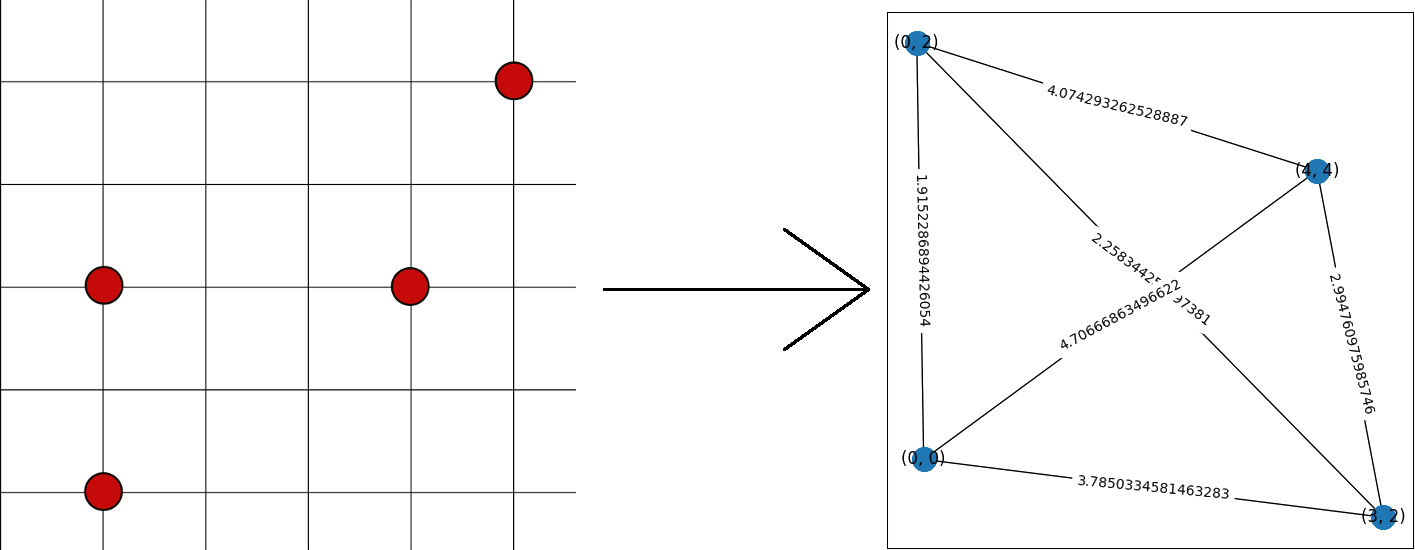
\includegraphics[width=\textwidth]{grapheSimp.png}
	\caption{Comme on connaît le chemin optimal entre chaque couple de points, et qu'on sait à l'avance par quels points on veut passer, on peut passer de la grilleà un graphe simplifié, dont les arêtes sont valuées en temps.}
	\label{fig:grapheSimp}
\end{figure}
\subsection{Application d'un Dijkstra simplifié}
\paragraph{L'algorithme de Dijkstra}
L'algorithme de Dijkstra s'applique à un graphe non orienté dont toutes les arêtes ont un poids. Il a pour but de trouver le chemin le plus court entre un sommet de départ et un sommet d'arrivée. En langage naturel, l'algorithme de Dijkstra peut être décrit ainsi:
\begin{itemize}
	\item A chaque sommet est associée une distance au sommet de départ, qu'on appelera la "distance à 0". Initialement, on met tous les sommets à l'infini (sauf le sommet de départ, qui est à 0 de lui-même).
	\item A chaque sommet, on associe l'attribut "non visité".
	\item Il faut choisir un sommet, qu'on appelera le sommet "en cours". On choisit le sommet initial.
	\item Tant qu'une des conditions d'arrêt ci-dessous n'est pas atteinte:
	\begin{itemize}
		\item Pour chaque voisin non visité du sommet en cours:
			\begin{itemize}
				\item Calculer une nouvelle distance à 0 du voisin, en additionnant le poids de l'arête à la distance à 0 du sommet courant.
				\item Si la nouvelle distance à 0 du voisin est inférieure à la distance à 0 qui lui est actuellement associée, alors remplacer l'ancienne par la nouvelle. Sinon, garder l'ancienne.
			\end{itemize}
		\item Marquer le sommet en cours comme étant visité.
		\item Si le sommet de destination a été atteint, sortir de la boucle.
		\item Si la plus petite distance à 0 de l'ensemble des sommets non visités est l'infini, cela signifie qu'il n'existe aucun chemin passant par le sommet de départ et le sommet d'arrivée. Sortir de la boucle.
		\item Dans l'ensemble des sommets non visités, choisir celui dont la distance à 0 est minimale en tant que sommet en cours.
	\end{itemize}
	\item Maintenant que les distances à 0 ont été valuées, pour construire le plus court chemin, il suffit de partir du sommet de départ, et de choisir à chaque étape le voisin dont la distance à 0 est minimale.
\end{itemize}
\paragraph{Simplification de Dijkstra pour notre problème}
Il existe des différences entre notre problème et celui que Dijkstra résout:
\begin{itemize}
	\item Il faut passer par tous les sommets;
	\item Deux sommets peuvent être alignés ou non alignés dans la grille, et cela modifie le coût. Il y a donc un coût intrinsèque à l'arête, mais aussi un coût lié à un triplet (arête, sommet, arête).
	\item Le coût entre deux sommets du graphe simplifié est déjà considéré comme "raisonnable" donc on n'est pas dans la situation d'un voyageur de commerce (on peut se contenter d'une solution bonne mais non optimale).
	\item On a un graphe fortement connexe (ce qui n'est pas forcément le cas d'un problème de Dijkstra). En ignorant le point précédent, cela signifie qu'il suffit de construire le chemin en prenant toujours l'arête la plus légère pour trouver le chemin optimal.
\end{itemize}
Avec les adaptations mentionnées ci-dessus, on obtient l'algorithme qui a été implémenté dans notre prototype.
\subsection{Comparaison avec d'autres algorithmes et performances}
\paragraph{Autres algorithmes}
Pour tester notre méthode, nous avons également implémenté d'autres algorithmes connus:
\begin{itemize}
	\item Un algorithme génétique de voyageur de commerce;
	\item L'algorithme de Ford-Bellman.
\end{itemize}
Faute de temps, nous n'avons pu les tester expérimentalement, mais ils sont déjà prêts à l'usage dans le code que nous avons livré.
\paragraph{Complexité}
\begin{itemize}
	\item En ce qui concerne la complexité en mémoire, comme nous l'avons mentionné, notre graphe simplifié possède $\frac{n(n-1)}{2}$, donc l'ordre est $O(n^2)$ où $n$ est le nombre de points d'arrêt imposé.\\
	\item Pour la complexité en temps, l'algorithme est séparé en deux parties:
	\begin{itemize}
			\item La valuation des chemins optimaux dans les sous-grille, en $O(n^2)$ (une opération par arête du graphe simplifié).
			\item Le calcul du chemin optimal, en $O(n)$ dans le meilleur des cas et en $O(n^2)$ dans le pire des cas.
	\end{itemize}
\end{itemize}
